%Talk given virtually for SIAM UQ 2020 March
\documentclass[10pt,compress,xcolor={usenames,dvipsnames},aspectratio=169]{beamer}
%\documentclass[xcolor={usenames,dvipsnames},aspectratio=169]{beamer} %slides and 
%notes
\usepackage{amsmath,
	amssymb,
	datetime,
	mathtools,
	bbm,
	%mathabx,
	array,
	booktabs,
	xspace,
	calc,
	colortbl,
	siunitx,
 	graphicx}
\usepackage[usenames]{xcolor}
\usepackage[giveninits=false,backend=biber,style=nature, maxcitenames =10, mincitenames=9]{biblatex}
\addbibresource{FJHown23.bib}
\addbibresource{FJH23.bib}
\usepackage{newpxtext}
\usepackage[euler-digits,euler-hat-accent]{eulervm}
\usepackage{media9}
\usepackage[autolinebreaks]{mcode}
\usepackage[tikz]{mdframed}


\usetheme{FJHSlimNoFoot169}
\setlength{\parskip}{2ex}
\setlength{\arraycolsep}{0.5ex}

\DeclareMathOperator{\sol}{SOL}
\DeclareMathOperator{\app}{APP}
\DeclareMathOperator{\alg}{ALG}
\DeclareMathOperator{\ACQ}{ACQ}
\DeclareMathOperator{\ERR}{ERR}
\DeclareMathOperator{\COST}{COST}
\DeclareMathOperator{\COMP}{COMP}
\newcommand{\dataN}{\bigl(\hf(\vk_i)\bigr)_{i=1}^n}
\newcommand{\dataNj}{\bigl(\hf(\vk_i)\bigr)_{i=1}^{n_j}}
\newcommand{\dataNjd}{\bigl(\hf(\vk_i)\bigr)_{i=1}^{n_{j^\dagger}}}
\newcommand{\ERRN}{\ERR\bigl(\dataN,n\bigr)}

\newcommand{\Sapp}{S_{\textup{app}}}
\newcommand{\LambdaStd}{\Lambda^{\textup{std}}}
\newcommand{\LambdaSer}{\Lambda^{\textup{ser}}}
\newcommand{\LambdaAll}{\Lambda^{\textup{all}}}
\newcommand{\oton}{1\!:\!n}
\newcommand{\talert}[1]{\alert{\text{#1}}}
\DeclareMathOperator{\init}{init}
\DeclareMathOperator{\GP}{\cg\cp}
\newcommand{\MLE}{\textup{EB}}
\newcommand{\mCtheta}{{\mathsf{C}_{\vtheta}}}
\newcommand{\mCInv}{\mathsf{C}^{-1}}

%\DeclareMathOperator{\app}{app}

\providecommand{\HickernellFJ}{H.}


\iffalse
The Successes and Challenges of Automatic Bayesian Cubature

The promise of Bayesian cubature is that with reasonable prior information (or assumptions) about the integrand, one can construct an optimal approximation to the corresponding (multidimensional) integral and simultaneously a credible interval.  Automatic Bayesian cubature uses increases the sample size until half-width of the credible interval is small enough.  We discuss how to choose appropriate covariance kernels, estimate their hyper-parameters, and construct the credible intervals, all with reasonable computational effort.  We also evaluate the performance of automatic Bayesian cubature on a variety of examples.


\fi

\renewcommand{\OffTitleLength}{-10ex}
\setlength{\FJHThankYouMessageOffset}{-8ex}
\title{The Successes and Challenges of Automatic Bayesian Cubature}
\author[]{Fred J. Hickernell}
\institute{Department of Applied Mathematics \\
	Center for Interdisciplinary Scientific Computation \\  Illinois Institute of Technology \\
	\href{mailto:hickernell@iit.edu}{\url{hickernell@iit.edu}} \quad
	\href{http://mypages.iit.edu/~hickernell}{\url{mypages.iit.edu/~hickernell}}}

\thanksnote{with Jagadeeswaran R. and the GAIL team \\
	partially supported by  NSF-DMS-1522687 and NSF-DMS-1638521 (SAMSI) \\[2ex]
	Thanks to the special session organizers
	
}
\event{SIAM-UQ 2020}
\date[]{March 2020}

\input FJHDef.tex


\newlength{\figwidth}
\setlength{\figwidth}{0.25\textwidth}

\newlength{\figwidthSmall}
\setlength{\figwidthSmall}{0.2\textwidth}

\newcommand{\financePict}{\href{http://i2.cdn.turner.com/money/dam/assets/130611131918-chicago-board-options-exchange-1024x576.jpg}{\includegraphics[width
		= 3cm]{ProgramsImages/130611131918-chicago-board-options-exchange-1024x576.jpg}}}
	
	\newcommand{\scoop}[1]{\parbox{#1}{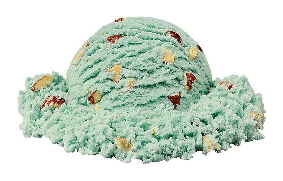
\includegraphics[width=#1]{IceCreamScoop.eps}}\xspace}
	\newcommand{\smallscoop}{\scoop{1cm}}
	\newcommand{\medscoop}{\scoop{1.8cm}}
	\newcommand{\largescoop}{\scoop{3cm}}
	\newcommand{\ICcone}[1]{\parbox{#1}{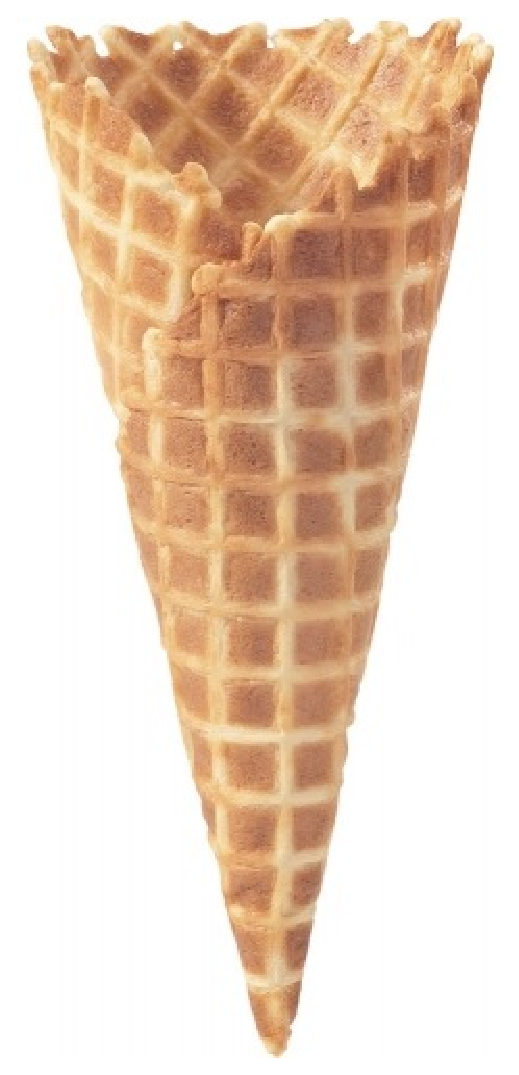
\includegraphics[width=#1,angle=270]{MediumWaffleCone.eps}}\xspace}
	\newcommand{\medcone}{\ICcone{1.2cm}}
	\newcommand{\largercone}{\parbox{2.2cm}{\vspace*{-0.2cm}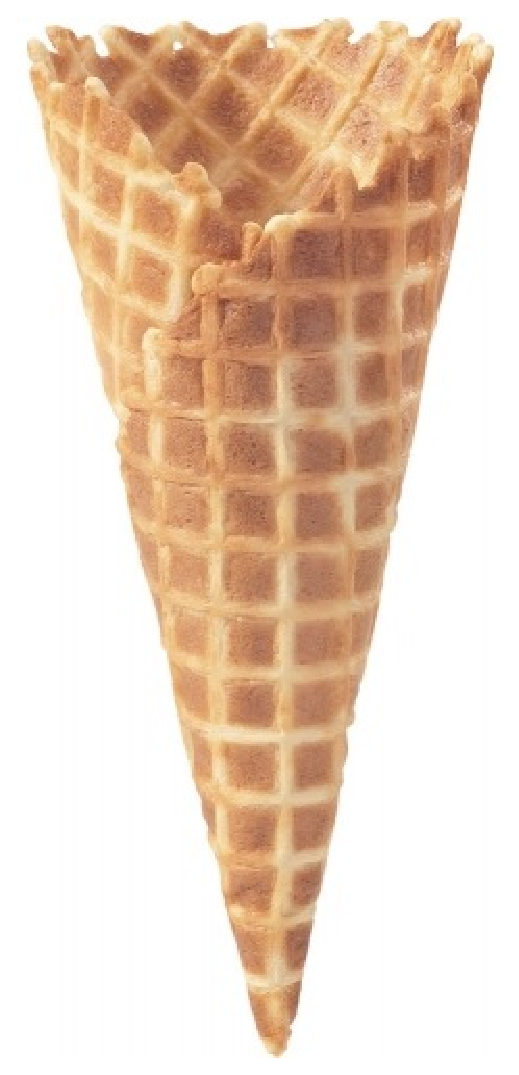
\includegraphics[width=1cm,angle=270]{MediumWaffleCone.eps}}\xspace}
	\newcommand{\largecone}{\ICcone{1.8cm}}
	\newcommand{\smallcone}{\parbox{1.1cm}{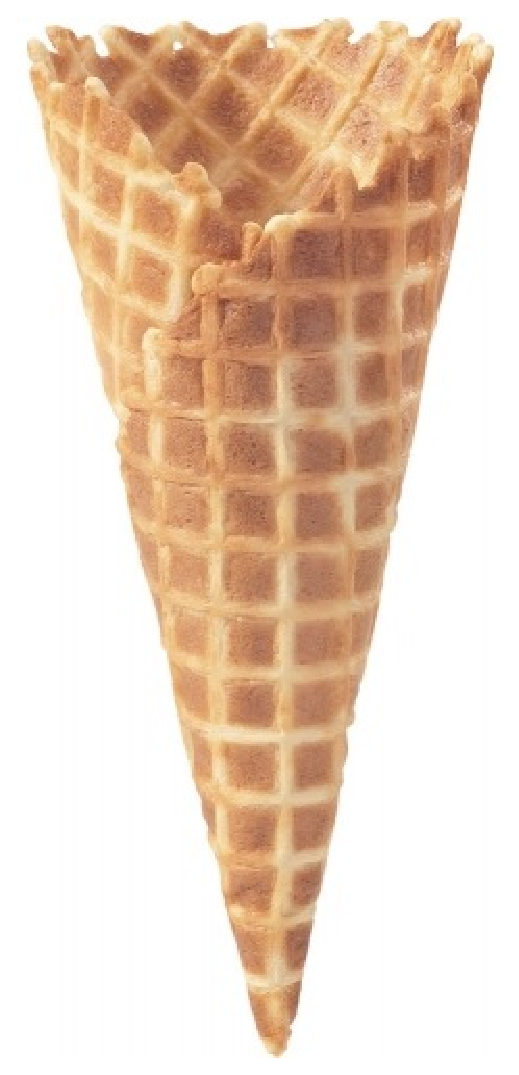
\includegraphics[width=0.5cm,angle=270]{MediumWaffleCone.eps}}\xspace}

	

\newcommand{\northeaststuff}[3]{
	\begin{tikzpicture}[remember picture, overlay]
	\node [shift={(-#1 cm,-#2 cm)}]  at (current page.north east){#3};
	\end{tikzpicture}}


\begin{document}
	\tikzstyle{every picture}+=[remember picture]
	\everymath{\displaystyle}

\frame{\titlepage}


\section{Introduction}

\begin{frame}
	{The Guaranteed Automatic Integration Library (GAIL) and QMCPy Teams}
	
	\vspace{-2ex}
	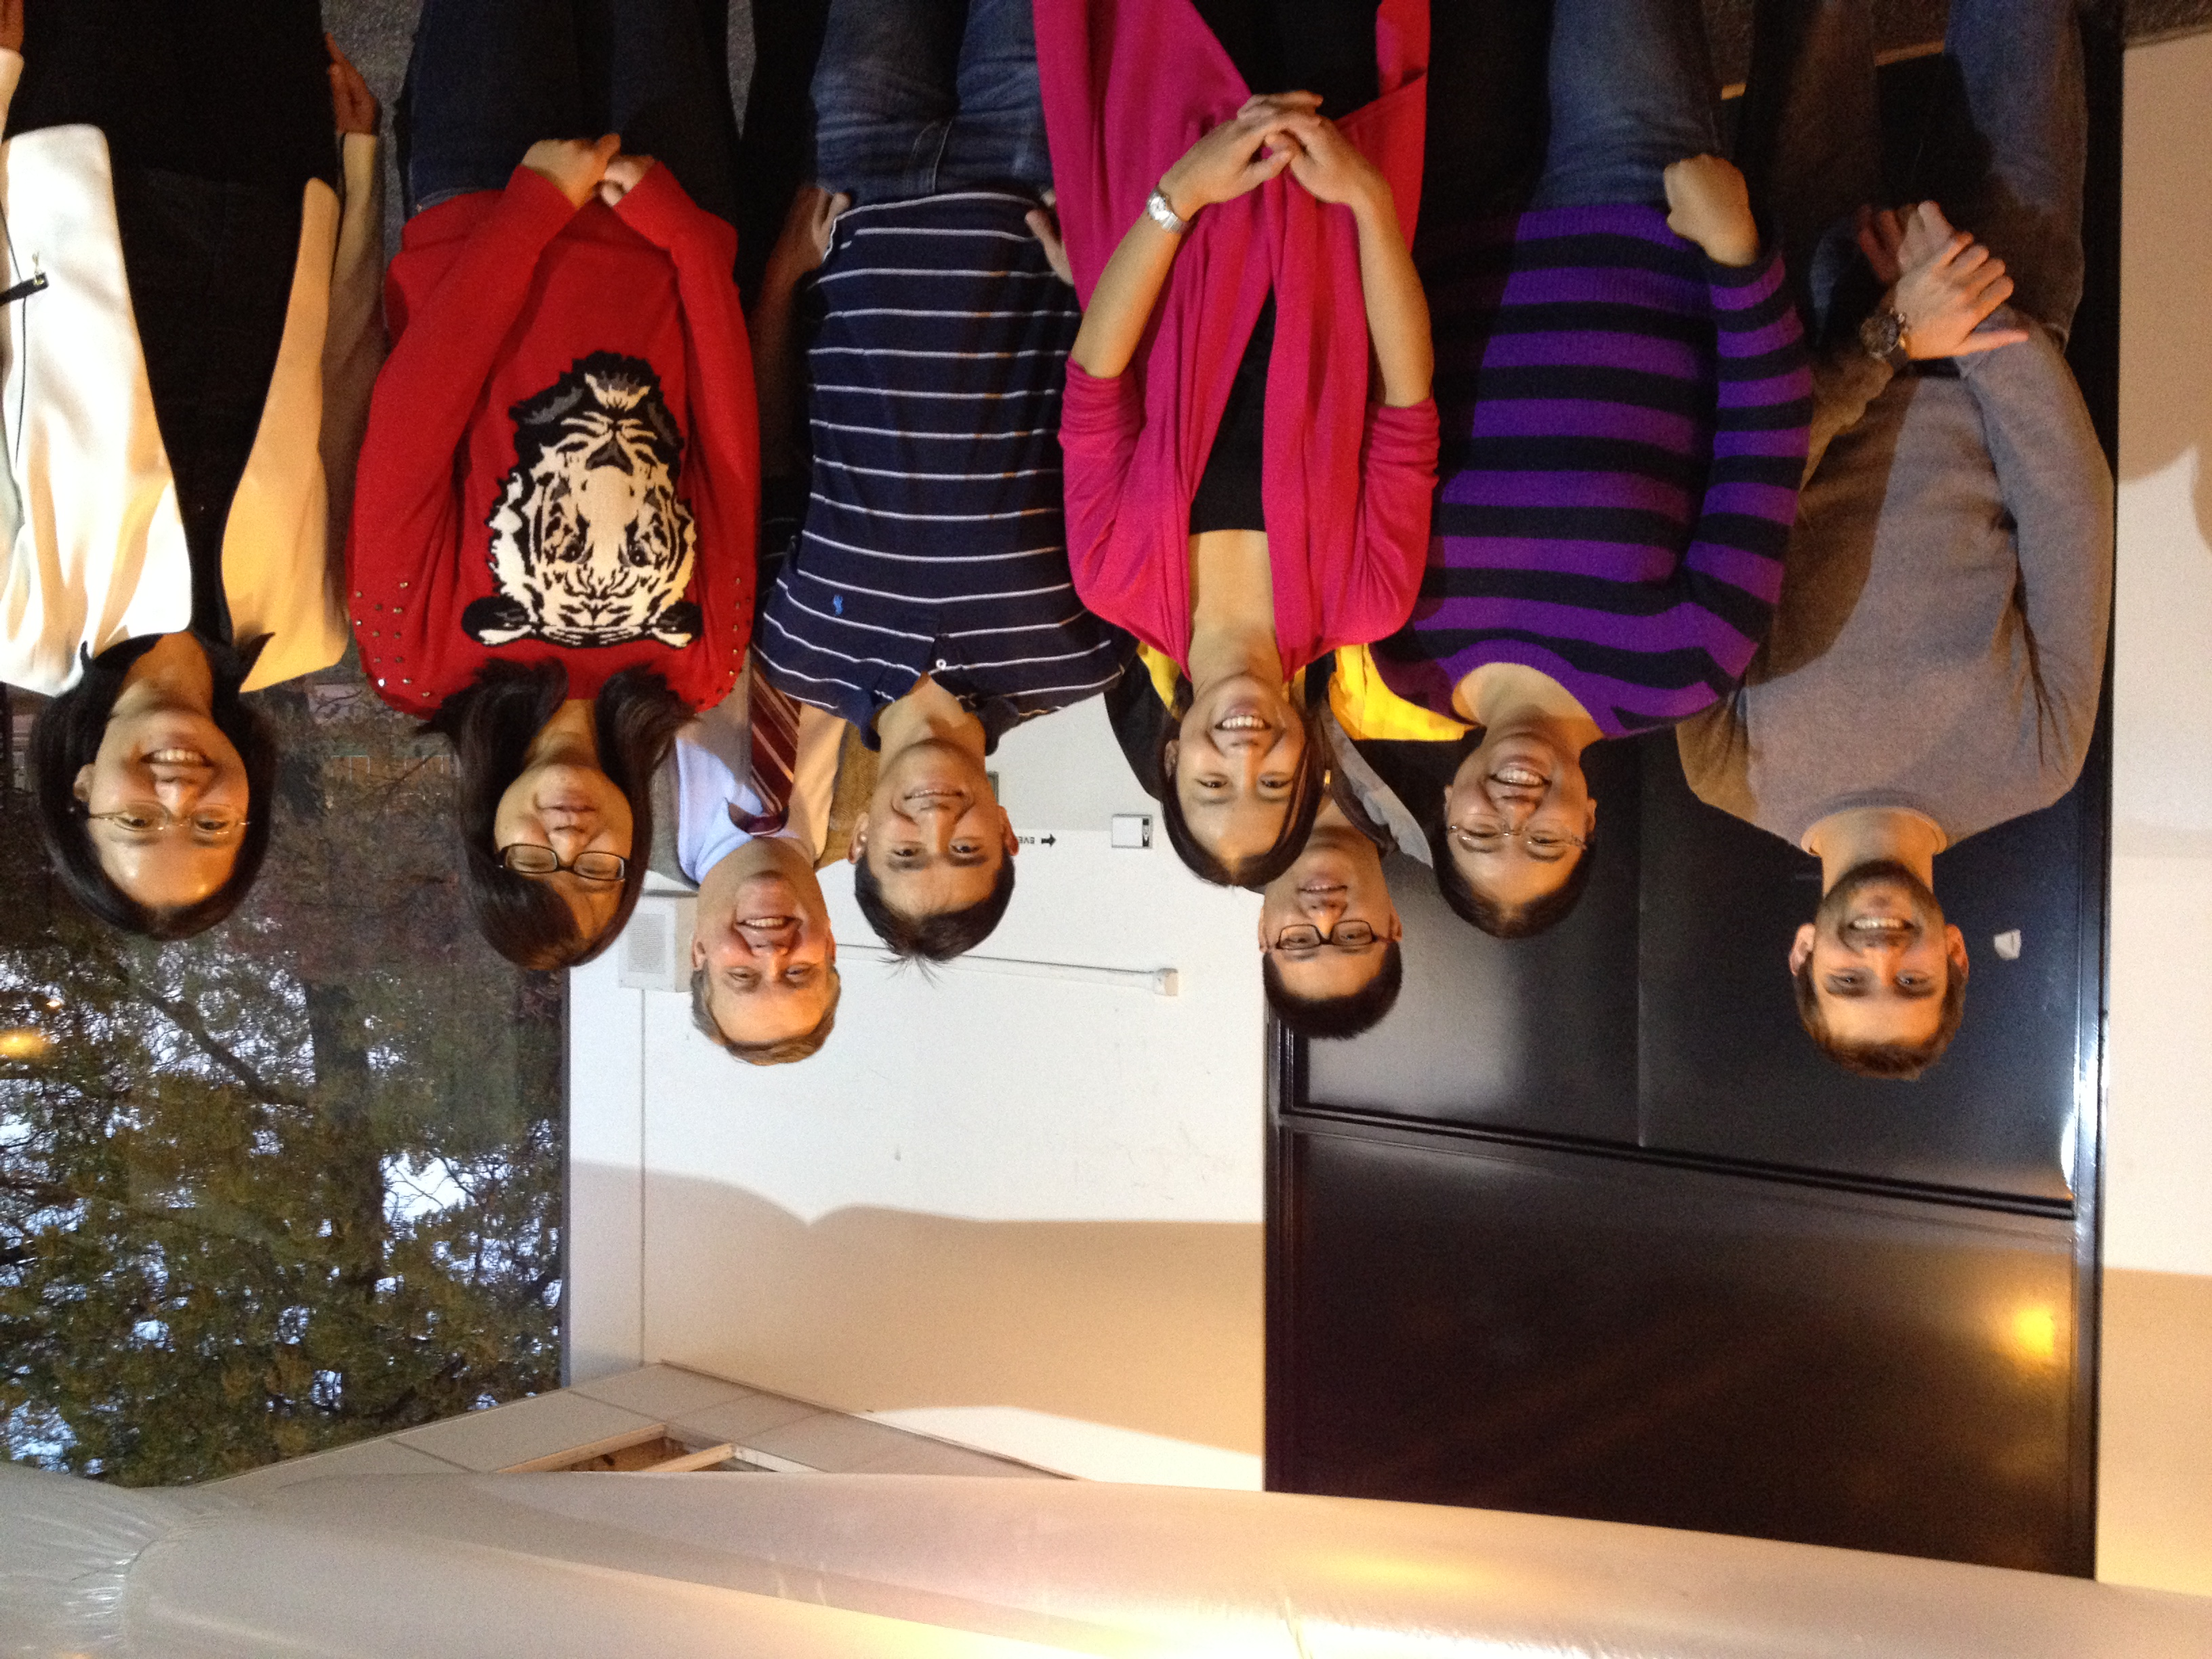
\includegraphics[angle = 180, origin = c, width = 0.32\textwidth]{ProgramsImages/GAIL2014RE.jpeg} \
	
\includegraphics[width = 0.32\textwidth]{ProgramsImages/GAILatSIAM2018Hi.jpeg} \ 
	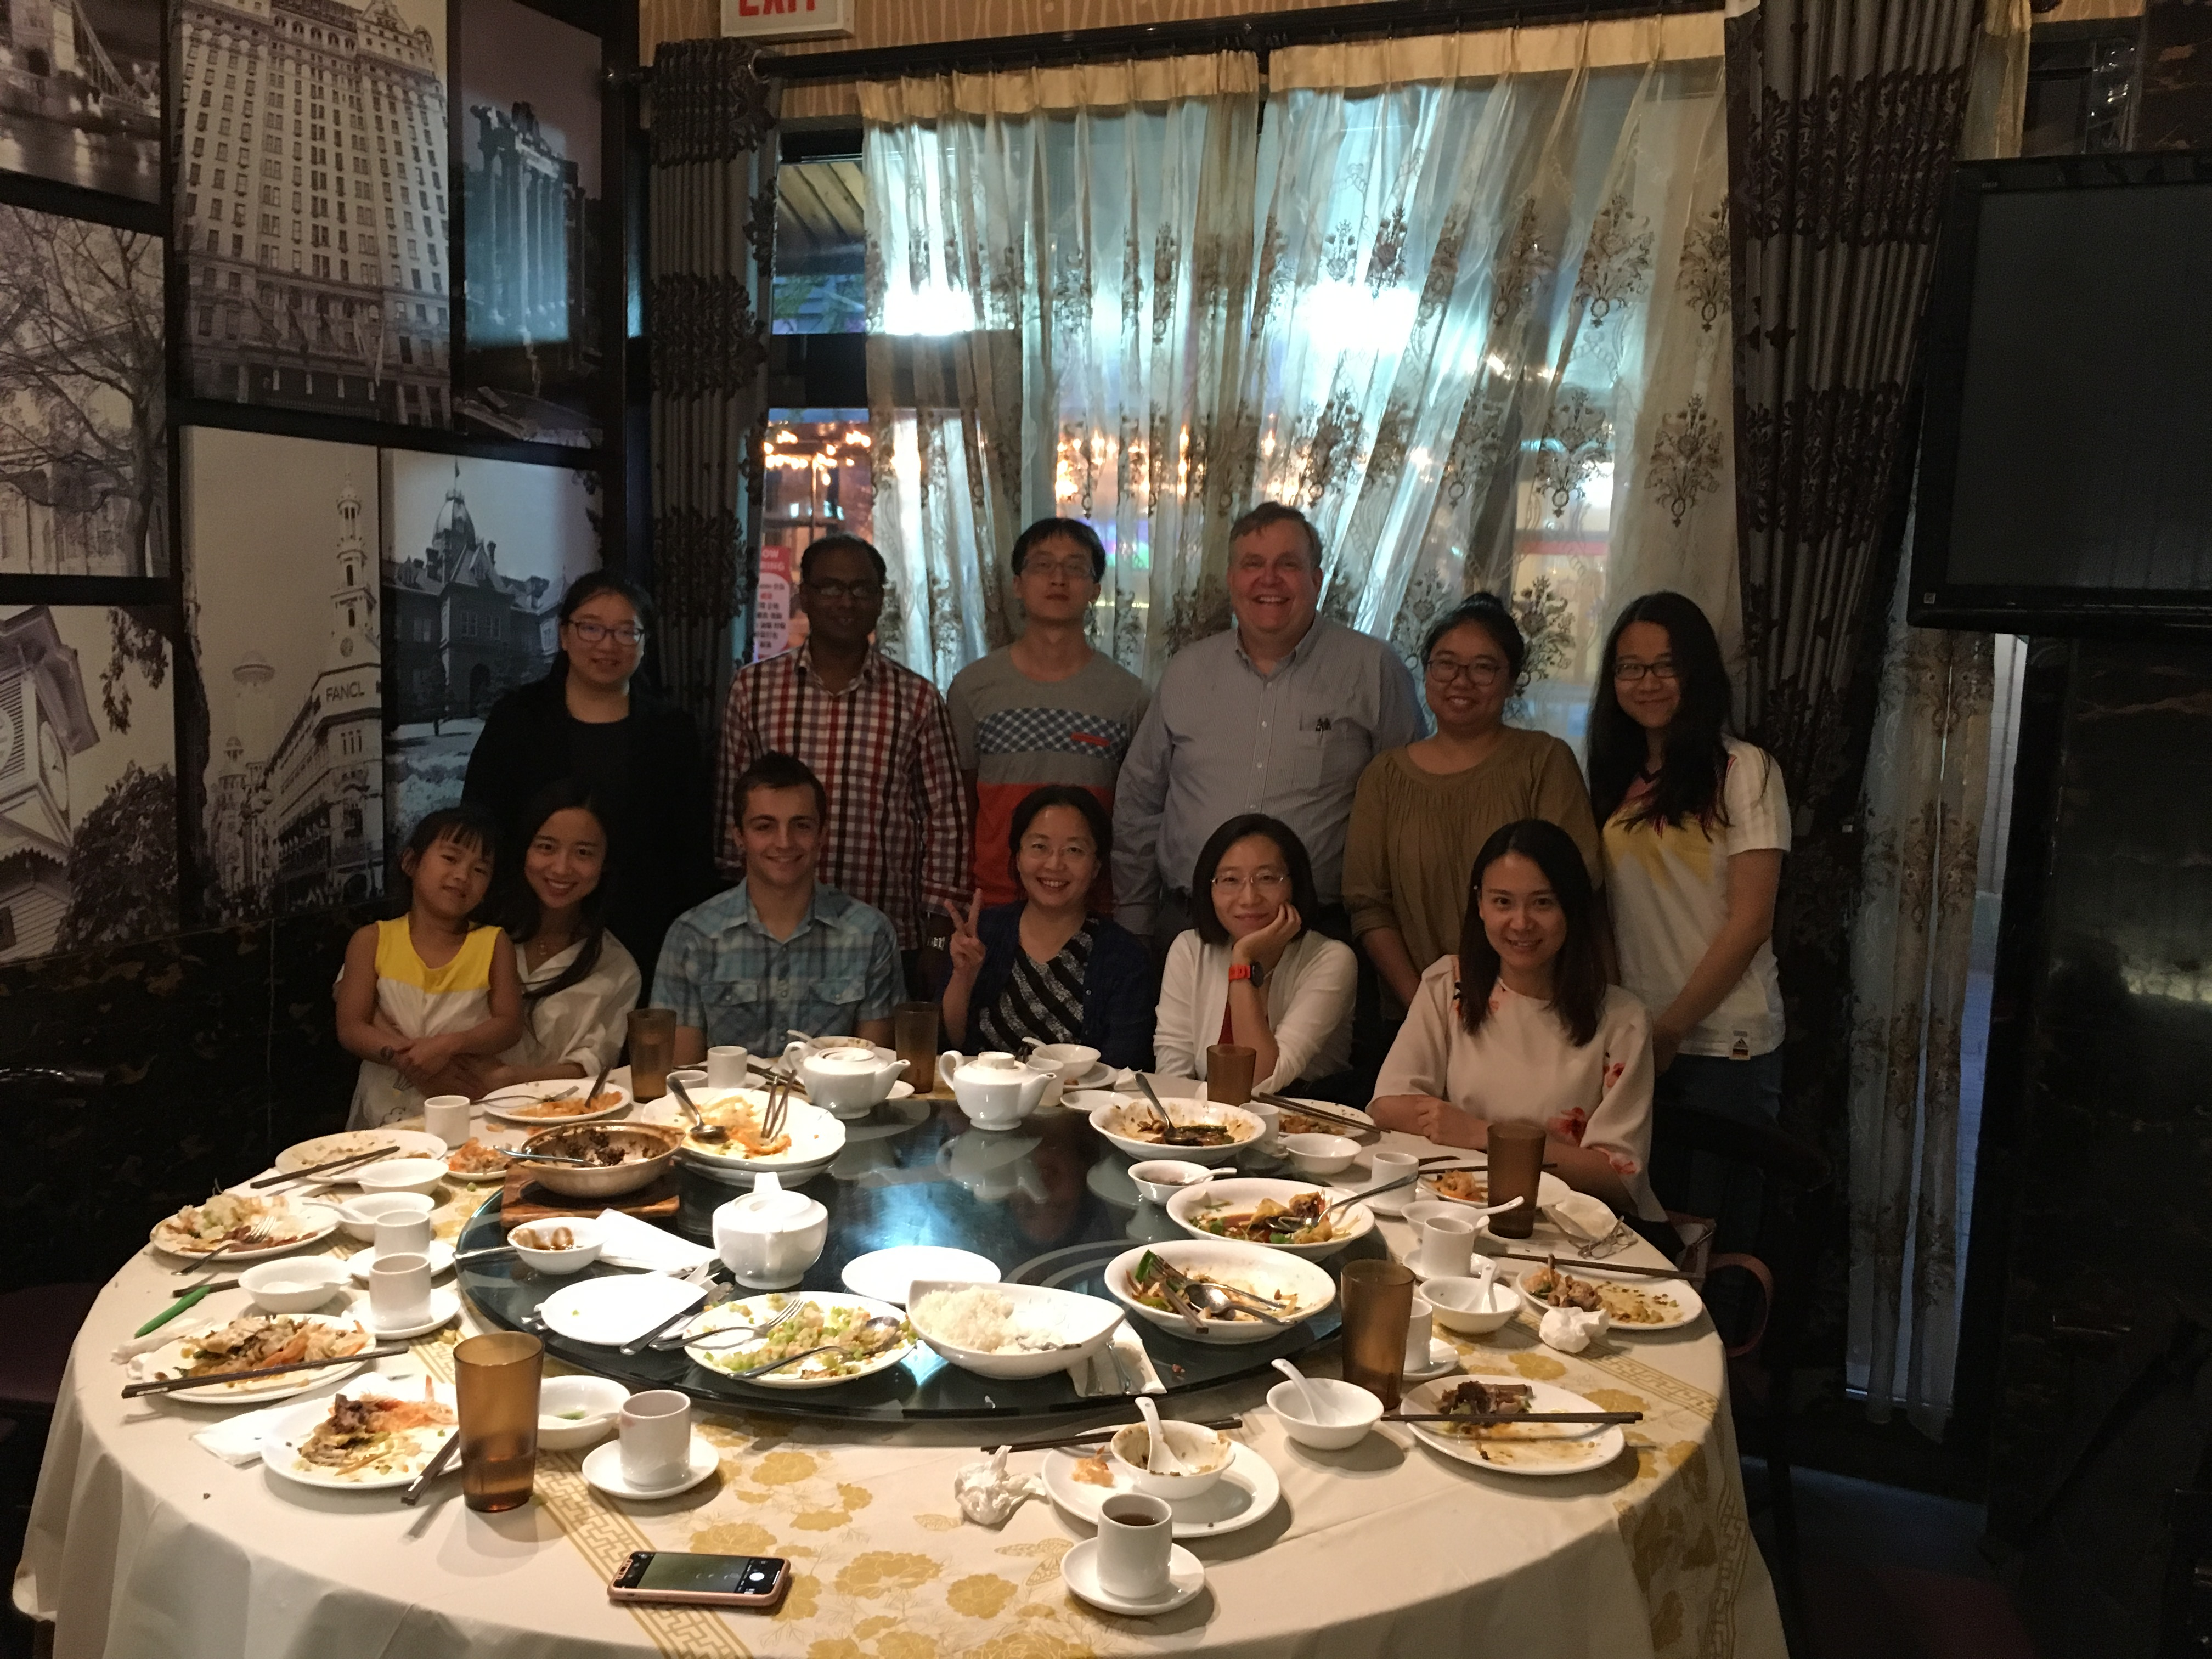
\includegraphics[width = 0.32\textwidth]{ProgramsImages/GAILatChinatown2018.jpg}
	
	\vspace{-3ex}
	\begin{tabular}{p{0.55\textwidth}p{0.42\textwidth}}
		
			
		\begin{itemize}
			\item Sou-Cheng Choi (Chief Data Scientist, Kamakura)
			
			\item Yuhan Ding (IIT PhD '15, Lecturer, IIT)
			
			\item Lan Jiang  (IIT PhD '16, Compass)
			
			\item Llu\'is Antoni Jim\'enez Rugama (IIT PhD '17, UBS)
			
			\item Jagadeeswaran Rathinavel (IIT PhD '19, Wi-Tronix)
			
			\item Aleksei Sorokin (IIT BS + MAS '21 exp.)
	
			
		\end{itemize}
	
	&
	
		\begin{itemize}
	
	
	\item Tong Xin (IIT MS, UIC PhD '20 exp.)
	
	\item Kan Zhang (IIT PhD '20 exp.)
	
	\item Yizhi Zhang (IIT PhD '18, Jamran Int'l)
	
	\item Xuan Zhou (IIT PhD '15, JP Morgan)
	
	\item and others
	
	
\end{itemize}

Adaptive software libraries \href{https://gailgithub.github.io/GAIL_Dev/}{\beamerbutton{GAIL}} and \href{https://qmcsoftware.github.io/QMCSoftware/}{\beamerbutton{QMCPy}}

	
	\end{tabular}
\end{frame}


\begin{frame}{Problem}
	\only<1-4>{\northeaststuff{1}{2.4}{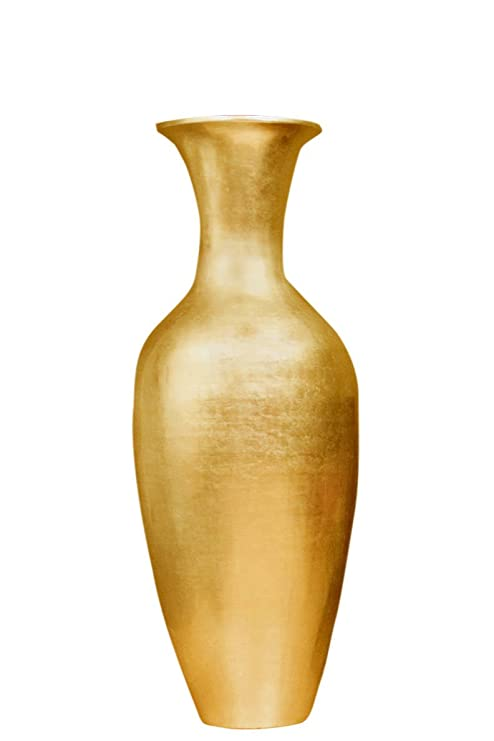
\includegraphics[width=2cm]{ProgramsImages/GoldVase.jpg}}}
	\only<5->{\northeaststuff{1}{2.4}{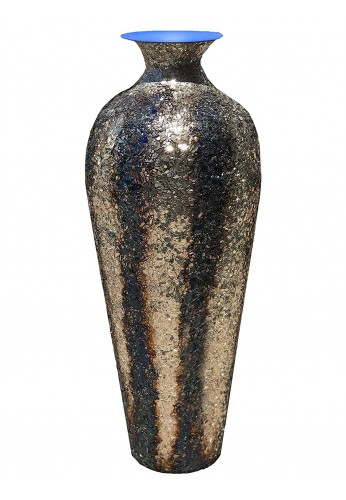
\includegraphics[width=2cm]{ProgramsImages/decorshore-fired-gold-vase-with-striped-crackled-glass-mosaic-vases.jpg}}}
	\northeaststuff{1}{0.9}{\alert{$f$}}

\vspace{-8ex}

   Want \alert{fixed tolerance cubature} $\alg: L^1[0,1]^d \times (0,\infty) \to \reals$ such that 
   
   \vspace{-4ex}
    \[
    \only<2->{\Prob_f \Bigg [ }\biggabs{\int_{[0,1]^d} f(\vx) \, \dif \vx - \alg(f,\varepsilon)} \le \varepsilon \only<2->{\Bigg ] \ge 99\%} \qquad \forall \varepsilon > 0, \quad \only<1>{\talert{for reasonable $f$}}\only<2->{\alert{f \sim \GP(m,s^2C_{\vtheta})}}
    \]
    \vspace{-3ex}
    \uncover<3->{\begin{gather*}
        \text{\alert{design or node array} }\mX = (\vx_1, \ldots, \vx_n)^T \in [0,1]^{n \times d}, \qquad \text{\alert{function data} }  \vf = f(\mX)\in \reals^n \\
    c_{0\vtheta} = \int_{[0,1]^{d} \times [0,1]^{d}} C_{\vtheta}(\vt,\vx) \, \dif \vt \dif \vx > 0, \quad 
\vc_\vtheta = \int_{[0,1]^{d}} C_{\vtheta}(\mX,\vt) \, \dif \vt \in [0,1]^{n} , \quad
\mC_\vtheta = C_{\vtheta}(\mX,\mX)  \in [0,1]^{n \times n} \\
\int_{[0,1]^d} f(\vx) \, \dif \vx  \, \big \vert \, (\vf = \vy) \sim \cn\Bigl(\underbrace{ m[ 1 - \vc_\vtheta^T \mC_\vtheta^{-1}\vone] + \vc_\vtheta^T \mC^{-1}\vy}_{\alg(f,\varepsilon)}, s^2(c_{0\vtheta} - \vc_\vtheta^T \mC_\vtheta^{-1}\vc_\vtheta)\Bigr)
    \end{gather*}
    
    \vspace{-4ex}
Choosing $n$  large enough to make $2.58s\sqrt{c - \vc^T \mC^{-1}\vc} \le \varepsilon$ would seem to achieve our goal

 
 \vspace{-1ex}
 \uncover<4->{
 	\alert{Issues requiring attention}
 	
 	\vspace{-3ex}
 \begin{itemize}
 	\item Inference of $m$, $s$,  $\vtheta$, and $C_{\vtheta}$, which urn  $f$ comes from
 	\item Ill-conditioning and numerical cost of vector-matrix calculations
 	\item Whether Gaussian process is a reasonable assumption
\end{itemize}}}
    
\end{frame}

\begin{frame}{Inferring Gaussian Process Parameters for $\GP(m,s^2C_{\vtheta})$\footfullcite{RatHic19a}}
\only<1->{\northeaststuff{1}{2.4}{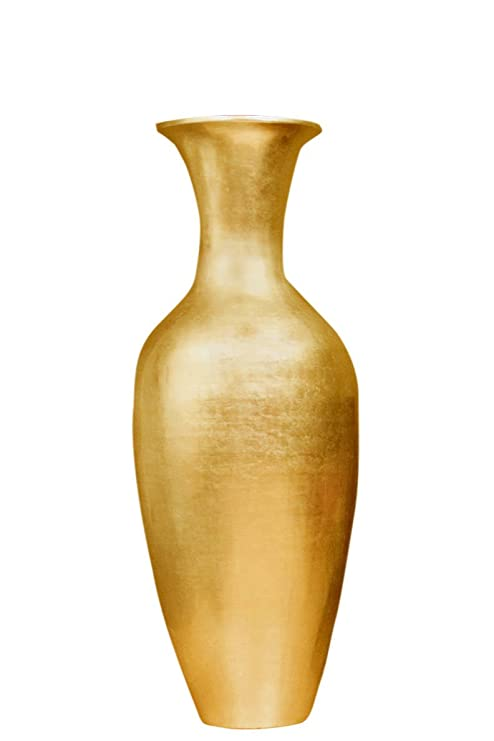
\includegraphics[width=2cm]{ProgramsImages/GoldVase.jpg}}}
\only<2->{\northeaststuff{1}{2.4}{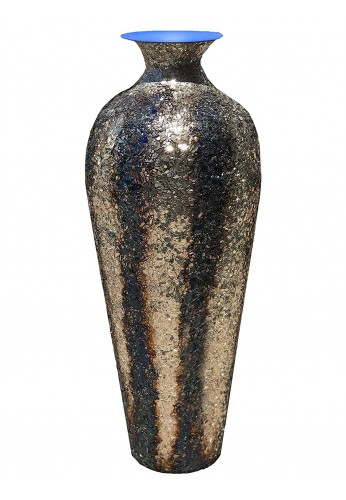
\includegraphics[width=2cm]{ProgramsImages/decorshore-fired-gold-vase-with-striped-crackled-glass-mosaic-vases.jpg}}}
\northeaststuff{1}{0.9}{\alert{$f$}}

\vspace{-10ex}

	Using \alert{empirical Bayes}
	\begin{gather*} 
m_{\MLE} = \frac{\vone^T \mCInv_\vtheta \vy }{ \vone^T \mCInv_\vtheta \vone}, \qquad
s^2_{\MLE} = 
\frac{1}{n}
\vy^T 
\left[ \mCInv_\vtheta - 
\frac{ \mCInv_\vtheta \vone \vone^T \mCInv_\vtheta }{\vone^T\mCInv_\vtheta \vone}
\right] \vy, \\
\vtheta_{\MLE}
= \argmin_{\vtheta} \biggl \{
\log\left(\vy^T 
\left[ \mC_\vtheta^{-1} - 
\frac{ \mCInv_\vtheta \vone \vone^T \mCInv_\vtheta }{\vone^T\mCInv_\vtheta \vone}
\right] \vy 
\right)  
+  \frac{1}{n} \log(\det(\mC_\vtheta))
\biggr \}, \\
\alg(f,\varepsilon) = 
\left(
\frac{ (1 - \vone^T  \mCInv_\vtheta\vc_{\vtheta} )  \vone }{ \vone^T \mCInv_\vtheta \vone}   +  \vc_{\vtheta} 
\right)^T  \mCInv_\vtheta \vy \qquad \text{when }
2.58 s_{\mathsf{\MLE}} \sqrt{c_{0\vtheta} - \vc_{\vtheta}^T\mC_\vtheta^{-1}\vc_{\vtheta} } \le \varepsilon
	\end{gather*}
	
	\vspace{-4ex}
	
\uncover<2->{\begin{itemize}
		\item Ill-conditioning and numerical cost of vector-matrix calculations
		\item Whether Gaussian process is a reasonable assumption
\end{itemize}}

\end{frame}

\section{Fast Bayesian Transforms}

\begin{frame}{Fast Bayesian Transforms in General}
	
	\vspace{-3ex} 
	
Find a kernel $C_\vtheta$ to \alert{match} the design $\mX$ so that

\vspace{-6ex}
\begin{gather*}
\mC_\vtheta = \frac 1n \mV \mLambda_\vtheta \mV^H , 
\quad \quad \mV^H = n \mV^{-1}, \qquad
\mV = (\vv_1,\ldots,\vv_n)^T = (\vV_1,\ldots,\vV_n) \text{ known analytically} \\
\vv_1 = \vV_1 = \vone, \qquad \vc_\vtheta = \vone, \qquad
	\widetilde{\vb} := \mV^H \vb  \text{ requires only $\Order(n \log(n))$ operations } \forall \vb.
\end{gather*}
$C_\vtheta$ is a \alert{fast Bayesian transform kernel} and $\vb \mapsto \mV^H \vb$ a \alert{fast Bayesian transform (FBT)} 

\vspace{-2ex}
Then by empirical Bayes
\begin{gather*}
\widetilde{\vy} = \talert{\,FBT of function data } \vy , \quad \vlambda_\vtheta = \diag(\mLambda_\vtheta) = (\lambda_{\vtheta,1} , \ldots, \lambda_{\vtheta,n})^T=  \widetilde{\vC}_{\vtheta,1} = \talert{\,FBT of first column of } \mC_\vtheta \\
	\vtheta_{\MLE} = 
\argmin_{\vtheta}
\left[
\log\left(
\sum_{i=\alert{2}}^n \frac{\abs{\widetilde{y}_i}^2}{\lambda_{\vtheta, i}}
\right) 
+ \frac{1}{n}\sum_{i=1}^n \log(\lambda_{\vtheta,i})
\right]\\
\alg(f,\varepsilon) =  \frac{\widetilde{y}_1}{n} = \frac 1n \sum_{i=1}^n y_i = \talert{ sample mean}
\qquad \text{when }
\frac{2.58}{n}\sqrt{
	\sum_{i=2}^{n} \frac{\abs{\widetilde{y}_i}^2}{\lambda_{\vtheta,i}}  
	\,
	\left( 1 -  \frac{n}{\lambda_{\vtheta,i}} \right) 
} \le \varepsilon
\end{gather*}
Cost is \alert{$O(n \log (n))$} times the number of iterations for optimizing $\vtheta$

\end{frame}

\begin{frame}{Types of FBT Kernels}
	
	\vspace{-6ex}
	\begin{tabular}{>{\centering}p{0.47\textwidth}@{\qquad}>{\centering}p{0.47\textwidth}}
		\multicolumn{2}{>{\centering}p{\textwidth}}{$C_\vtheta(\vt,\vx) = K_\vtheta(\vx \ominus \vt)$, \quad
			$\{\vx_i\}_{i=1}^{2^m} = $ affine shift of a group under $\oplus$ for $m = 0, 1, \ldots$} \tabularnewline
		\uncover<2->{Shifted Lattice Nodes, $\oplus = $ addition $\bmod \vone$} & 
	\uncover<2->{Scrambled Sobol' Nodes, $\oplus = $ bitwise addition}  \tabularnewline
		\uncover<2->{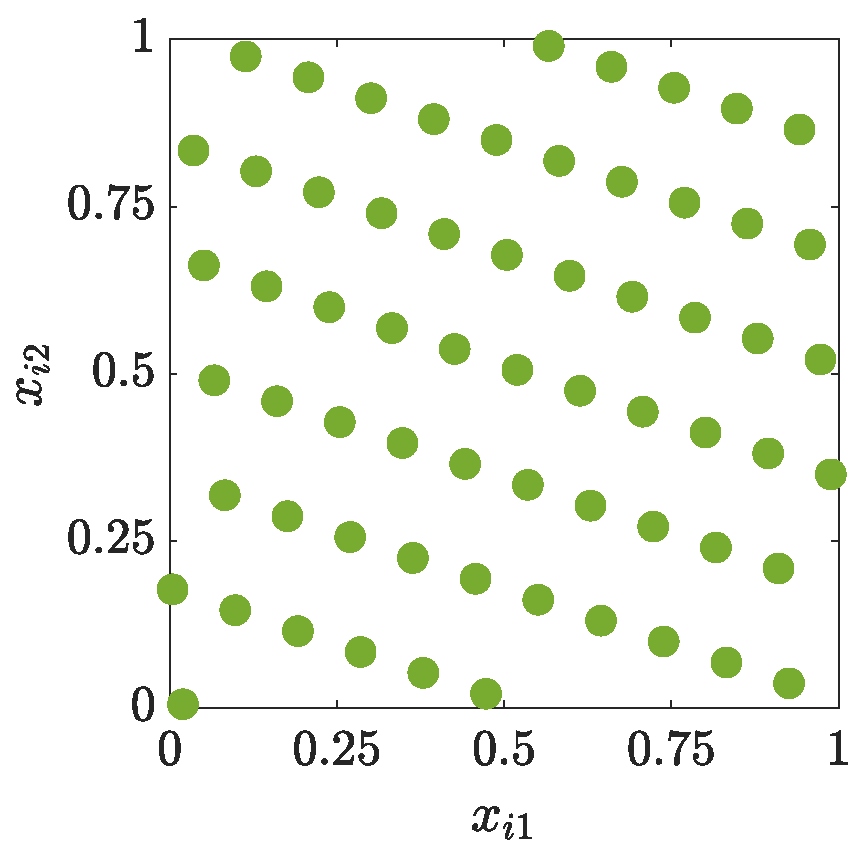
\includegraphics[height = 4cm]{ProgramsImages/ShiftedLatticePoints.eps}} &
		\uncover<2->{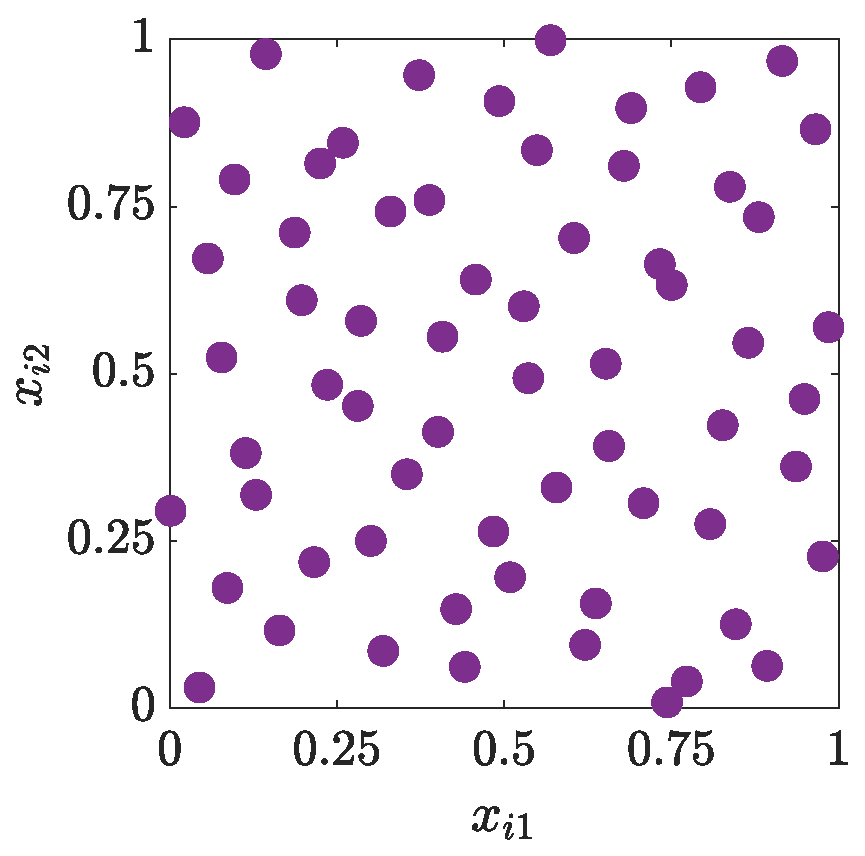
\includegraphics[height = 4cm]{ProgramsImages/SSobolPoints.eps}} \tabularnewline
		\uncover<3->{FBT  $ = $ \alert{Fast Fourier Transform}} &
			\uncover<3->{FBT $ = $ \alert{Fast Walsh Transform}}
	\end{tabular}
\end{frame}

\begin{frame}[label=flexible]{Flexible FBT Kernel for Lattice Node Designs}
	
\vspace{-4ex}

$C_\vtheta(\vt,\vx) = K_\vtheta(\vx \ominus \vt)$ must be \alert{positive definite}, where
$\oplus = $ addition $\bmod \vone$.  Common example is 

\vspace{-6ex}
\begin{align*}
K_\vtheta(\vx) & = \prod_{j=1}^d [1 + a' B_{2r'}(x_j)] = \prod_{j=1}^d [1 + a \kappa_r(x_j)], \qquad
\vtheta = (a,r) \in (0,\infty) \times (1,\infty), \quad r = 2r'\\
\kappa_r(x) &   : = \sum_{\abs{k} \ge 1}\frac{\exp(2\pi\sqrt{-1} kx)}{\abs{k}^{r}} \qquad
   \text{$B_{2r'}$ closed form, \alert{but $r' \in \naturals$},\quad $\kappa_r$ defined for  $r>1$, \alert{but infinite sum}}
\end{align*}

\uncover<2->{\alert{But} all we need to compute the integral and credible interval is $\widetilde{\vy}$ and 
	\[
	\vlambda_\vtheta =  \widetilde{\vC}_{\vtheta,1}, \qquad \text{where } \vC_{\vtheta,1} = \Bigl(  K_{\vtheta}(\vx_i \ominus \vx_1)\Bigr)_{i=1}^n,  \text{ which only depends on } \kappa_r(\ell/n) \text{ for } \ell = 0, \ldots, n-1
	\]
\uncover<3->{Moreover, $\bigl( \kappa_r(\ell/n) \bigr)_{\ell = 0}^{n-1}$ can be computed using \alert{one FFT} \hyperlink{kappaDeriv}{\beamergotobutton{details}}
}}

\end{frame}



\section{Numerical Examples}

 \begin{frame}[label=GaussProb]
	\frametitle{Keister's Example\footfullcite{Kei96}}
	\vspace{-6ex}
	\begin{tabular}{m{0.7\textwidth}m{3cm}}
		\begin{equation*}
		\int_{\reals^d} \cos(\norm{\vt})\exp(-\norm{\vt}^2) \, \dif \vt
		= \ \int_{[0,1]^{d-1}} 
		f(\vx) \, 
		\dif \vx 
		\end{equation*}
		& 
		%\includegraphics[height = 2.3cm]{Programs/GenzFun.eps}
	\end{tabular}
	
	\vspace{-4ex}
	
	\input{ProgramsImages/KeisterBayesOut.txt}
	
	\vspace{-4ex}
	
	Algorithms are implemented in GAIL\footfullcite{ChoEtal17b} and soon QMCPy\footfullcite{QMCPy2020a}
	
\end{frame}

 
 \begin{frame}[label=GaussProb]
 	\frametitle{Gaussian Probability\footfullcite{Gen93}}
 	\vspace{-8ex}
 	\begin{tabular}{m{0.7\textwidth}m{3cm}}
 		\begin{equation*}
 		\int_{(\va,\vb)} \frac{\exp\bigl(- \frac 12 \vt^T \mSigma^{-1} \vt 
 			\bigr)}{\sqrt{(2 
 				\pi)^d \det(\mSigma)}} \, \dif \vt \
 		= \ \int_{[0,1]^{d-1}} 
 		f(\vx) \, 
 		\dif \vx \qquad \talert{by Genz's transformation}
 		\end{equation*}
 		& 
 		%\includegraphics[height = 2.3cm]{Programs/GenzFun.eps}
 	\end{tabular}
 	 	
 	\vspace{-4ex}
 	
\input{ProgramsImages/MVNBayesOut.txt}

 	\vspace{-2ex}
 	
 Algorithms are implemented in GAIL\footfullcite{ChoEtal17b} and soon QMCPy\footfullcite{QMCPy2020a}
 
 
 
\end{frame}


\section{Gaussian Process Diagnostics}

\begin{frame}{Is $f$ a Typical Instance of a Gaussian Process?}
	
	\vspace{-2ex}
If $f \in \GP(m,s^2C_\vtheta)$, then 
$\vZ := s^{-1} \underbrace{n^{-1}\mV \mLambda_\vtheta^{-1/2} \mV^H}_{\mC_{\vtheta}^{-1/2}} ( \vf - m\vone) \sim \cn(\vzero,\mI)$.  
Generate the data 

\vspace{-4ex}
\[
\vz = \frac{1}{n s_{\MLE} } \mV \mLambda_{\vtheta_{\MLE}}^{-1/2} \mV^H ( \vy - m_{\MLE}\vone) = 
\left[\sum_{i=2}^n \frac{\abs{\widetilde{y}_i}^2}{\lambda_{\vtheta_{\MLE},i}} \right]^{-1} \mV \mLambda_{\vtheta_{\MLE}}^{-1/2} ( \widetilde{\vy} - \widetilde{y}_1 \ve_1)
\]

\vspace{-2ex}
\begin{tabular}{m{0.53\textwidth}>{\centering}m{0.44\textwidth}}
\alert{Q-Q plots} of $\vz$ vs.\ standard Gaussian

\bigskip

\uncover<2->{%
	\only<1-8>{\alert{Random function} fitting kernel with given $r$, $\theta$
\[
\begin{aligned}
f(\vx) & = \widehat{f}_0  \\
& + \sum_{\vk \in \{1, \ldots, N\}^d} \Bigl[\widehat{f}_c(\vk) \cos(2\pi \vk^T \vx) + \widehat{f}_s(\vk)\sin(2\pi \vk^T \vx)\Bigr] \\
& \qquad  \widehat{f}_0, \  \widehat{f}_c(\vk), \ \widehat{f}_s(\vk) \IIDsim \cn\biggl(0,a^{\norm[0]{\vk}} b^{d-\norm[0]{\vk}}\prod_{k_j \ne 0} k_j^{-r}\biggr) \\
& \qquad \theta = a/b,  \qquad N = 256
\end{aligned}
\]}%
\only<9->{$f$ from \alert{Keister's example}

\bigskip

True $r$ and $\theta$ unknown
}
}
&
\includegraphics<2>[width = 0.44\textwidth]{ProgramsImages/rand-QQPlot-n-64-d-2-r-150-th-25-1.eps}
\includegraphics<3>[width = 0.44\textwidth]{ProgramsImages/rand-QQPlot-n-64-d-2-r-150-th-25-2.eps}
\includegraphics<4>[width = 0.44\textwidth]{ProgramsImages/rand-QQPlot-n-64-d-2-r-150-th-100-1.eps}
\includegraphics<5>[width = 0.44\textwidth]{ProgramsImages/rand-QQPlot-n-64-d-2-r-150-th-100-2.eps}
\includegraphics<6>[width = 0.44\textwidth]{ProgramsImages/rand-QQPlot-n-64-d-2-r-400-th-400-1.eps}
\includegraphics<7>[width = 0.44\textwidth]{ProgramsImages/rand-QQPlot-n-64-d-2-r-400-th-400-2.eps}
\includegraphics<8>[width = 0.4\textwidth]{ProgramsImages/rand-rthInfer-n-64-d-2.eps}
\includegraphics<9>[width = 0.4\textwidth]{ProgramsImages/Keister-QQPlot-n-64-d-3-1.eps}
\includegraphics<10>[width = 0.4\textwidth]{ProgramsImages/Keister-QQPlot-n-64-d-3-2.eps}
\includegraphics<11>[width = 0.4\textwidth]{ProgramsImages/Keister-rthInfer-n-64-d-3.eps}
\includegraphics<12>[width = 0.4\textwidth]{ProgramsImages/Keister-QQPlot-n-1024-d-3-1.eps}
\includegraphics<13>[width = 0.4\textwidth]{ProgramsImages/Keister-QQPlot-n-1024-d-3-2.eps}
\includegraphics<14>[width = 0.4\textwidth]{ProgramsImages/Keister-rthInfer-n-1024-d-3.eps}
\end{tabular}

\end{frame}

\section{Summary}

\vspace{-6ex}

\begin{frame}
	{The Successes of Bayesian Cubature}
\northeaststuff{1}{2.4}{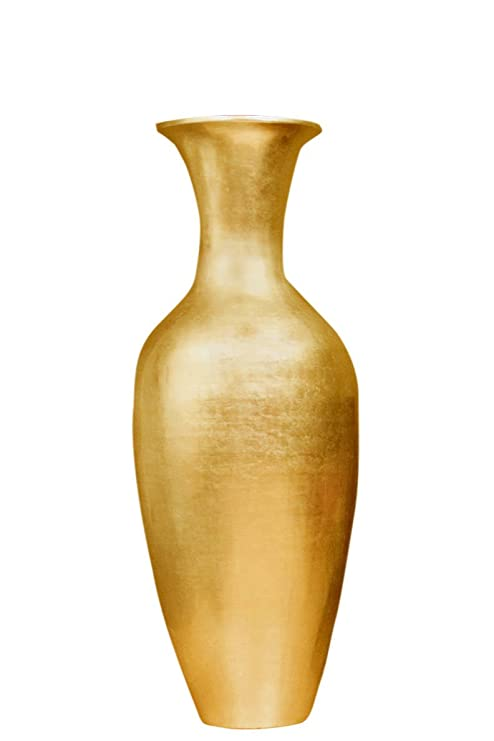
\includegraphics[width=2cm]{ProgramsImages/GoldVase.jpg}}
\northeaststuff{1}{0.9}{\alert{$f$}}

\vspace{-8ex}
	
\begin{minipage}{0.9\textwidth}

	\begin{itemize}
		\item \alert{Credible intervals} lead to adaptive cubature algorithms that provide answers to the desired tolerances
		
		\item \alert{Low discrepancy sampling} provides cubatures requiring fewer samples that IID sampling
		
		\item \alert{Empirical Bayes} and other methods can infer reasonable Gaussian process parameters for a family of covairance kernels---choosing a reasonable urn for $f$
		
		\item Covariance kernels that \alert{match} the low discrepancy sampling facilitate \alert{fast Bayeian transforms} for fitting the Gaussian process parameters,  computing the cubature, and constructing the credible intervals
		
		\item Extra effort provides a \alert{richer} family of covariance kernels
		
			
	\end{itemize}

\end{minipage}

\end{frame}


\begin{frame}
	{The Challenges of Bayesian Cubature}
	\northeaststuff{1}{2.4}{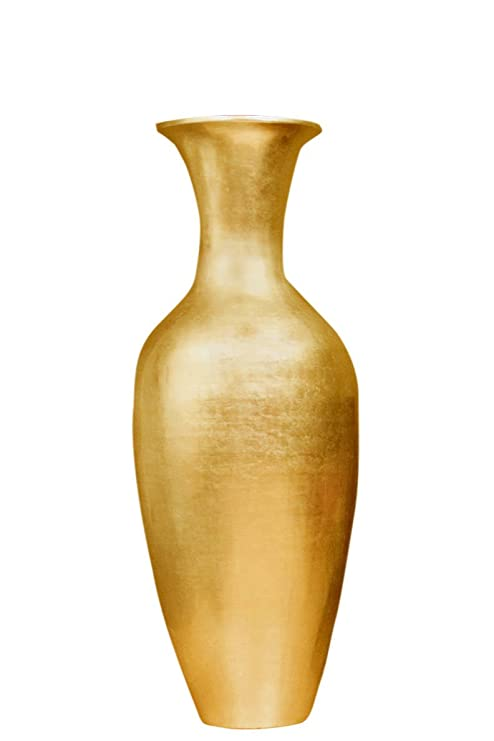
\includegraphics[width=2cm]{ProgramsImages/GoldVase.jpg}}
	\northeaststuff{1}{0.9}{\alert{$f$}}
	
	\vspace{-8ex}
	
	\begin{minipage}{0.9\textwidth}
		
		\begin{itemize}
			\item Inferring the Gaussian process parameters and allowing a larger family of kernels takes \alert{extra computational time}
			
			\item \alert{Overfitting} as well as underfitting the kernel are possible
			
			\item The \alert{Gaussian} assumption is not always justified by the data
			
			\item Which \alert{periodizing} transformations of $f$ are appropriate for lattice sampling and its matching kernels?
			
		\end{itemize}
		
	\end{minipage}
	
\end{frame}



\finalthanksnote{These slides are  available at \\  \href{https://speakerdeck.com/fjhickernell/right-ingredients-for-adaptive-function-approximation}{\nolinkurl{speakerdeck.com/fjhickernell/???}}}


\thankyouframe


\begin{frame}
	\frametitle{References}
\printbibliography
\end{frame}





\begin{frame}[label=kappaDeriv]{Computing $\kappa(x)$ for $x = 0, 1/n \ldots, 1-1/n$}
	\vspace{-8ex}
	\begin{align*}
	\zeta(s,a) &: = \sum_{m=0}^\infty (a+m)^{-s}  \quad \talert{Hurwitz zeta function}\\
	\kappa_r(\ell/n) & = \sum_{\abs{k} \ge 1} \frac{\exp(2\pi\sqrt{-1} k\ell/n)}{\abs{k}^{r}} 
	= \frac{2}{n^{r}}  \sum_{m=1}^\infty \frac{1}{\abs{m}^{r}} 
	+ 
	\sum_{k=1}^{n-1}  \sum_{m=-\infty}^{-\infty} \frac{\exp(2\pi\sqrt{-1} k\ell/n)}{\abs{k+mn}^{r}} 
	\\
	& = \frac{1}{n^{r}} \biggl\{2\zeta(r)
	+ 
	\sum_{k=1}^{n - 1} \exp(2\pi\sqrt{-1} k\ell/n) \bigl[ \zeta(r,k/n) + \zeta(r,1-k/n)\bigr] \biggr\} \\
	\vkappa_r & = \bigl( \kappa(\ell/n) \bigr)_{\ell = 0}^{n-1} = \mW^H \widetilde{\vkappa}_r \\
	\widetilde{\vkappa}_r & : = n^{-r}\bigl(2 \zeta(r), \zeta(r,1/n) + \zeta(r,(n-1)/n), \ldots, \zeta(r,(n-1)/n) + \zeta(r,1/n)  \bigr)^T \\
	\mW & = \bigl(\exp( 2 \pi \sqrt{-1} k \ell/n)\bigr)_{k,\ell =0}^{n-1}
	\end{align*}
	\hyperlink{flexible<3>}{\beamerreturnbutton{return}}
\end{frame}

\end{document}


\begin{frame}{What Should $\fC(\mX)$ Be?}
	\[
	\cc  =  \bigl\{ f \in \cf :  \norm[\cf]{f - \app(\mX,\vy)} \le  \alert{\fC(\mX)} \norm[\cf]{f} \bigr\}
	\]
	As $\mX$ covers $\cx$ better, $\fC(\mX)$ should decrease.  Suggest choosing
	\begin{align*}
	\frac{ \norm[\cf]{f - \app(\mX,\vy)}^2 }{ \norm[\cf]{f}^2 } = \fC^2(\mX) & : = \fC_0^2 \norm[\infty]{\frac{\sup \{ \abs{f(\cdot)}^2 : \norm[\cf]{f} \le 1,   \ f(\mX) = \vzero  \}}{\sup \{ \abs{f(\cdot)}^2 : \norm[\cf]{f} \le 1 \}}} \\
	&  = \fC_0^2  \norm[\infty]{\frac{K(\cdot,\cdot) -  K(\cdot,\mX)\bigl(K(\mX,\mX) \bigr)^{-1} K(\mX, \cdot)}{K(\cdot,\cdot)}}
	\end{align*}
	
	
\end{frame}


